\section{Grundlagen des Protokolls}
\label{sec:grundlagen_des_protokolls}


Um die Peer-to-Peer Funktionalität für das Protokoll dieser Arbeit zu gewährleisten, wird ein mehrschichtiges Verfahren verwendet. Für den effizienten Aufbau einer Direktverbindung zwischen zwei Teilnehmern kamen Chord und Kademlia in die engere Auswahl, welche beide lange Gegenstand intensiver Forschung waren, sowohl in der Industrie als auch in der akademischen Welt \parencite[S. 808]{MedranoChavez_ChordKademliaHighChurnScenarios}. 
Das Chord-Protokoll und das Kademlia-Protokoll sind zwei grundlegend verschiedene Ansätze zur Organisation von Peer-to-Peer-Netzwerken. Beide Protokolle sind strukturiert und bieten eine effiziente Ressourcenlokalisierung, aber sie unterscheiden sich in ihrer Routing-Struktur und der Art und Weise, wie sie die Knoteninformationen verwalten.

Chord basiert auf einer Ringstruktur (siehe Abbildung \ref{chord_ring}), bei der die Knoten in einem Ring angeordnet sind und jeder Knoten für einen bestimmten Schlüsselbereich verantwortlich ist. Die Verbindungen zwischen den Knoten sind durch ihren Platz im Ring definiert, wobei jeder Knoten eine Verbindung zu seinem nächsten Nachbarn im Uhrzeigersinn hat. Bei der Suche nach einem bestimmten Schlüssel durchläuft eine Anfrage einen logarithmischen Pfad im Ring, wobei die Knoten auf dem Weg begrenzte Informationen über andere Knoten behalten, um Anfragen weiterzuleiten. Dieses Modell ist recht einfach und effizient für viele Anwendungsfälle, aber es könnte anfällig sein für Engpässe oder längere Suchzeiten, insbesondere wenn das Netzwerk dynamisch ist und sich die Konfiguration häufig ändert.

\begin{center}
    \captionsetup{type=figure}
    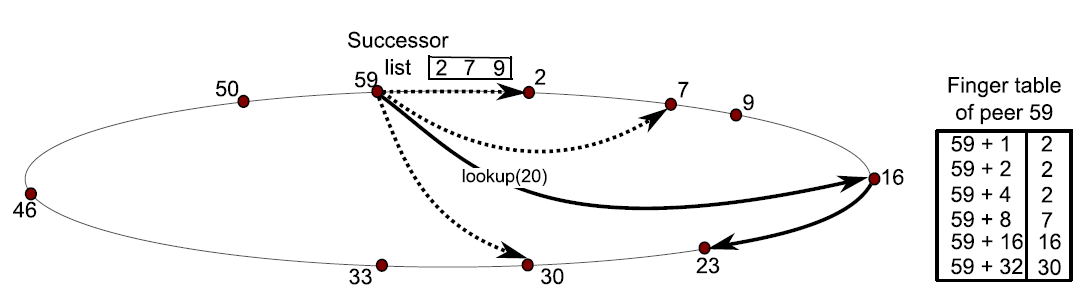
\includegraphics[width=0.9\linewidth]{images/chord_ring.png}
    \captionof{figure}{Visualisierung der Ringstruktur von Chord \parencite{MedranoChavez_ChordKademliaHighChurnScenarios}}
    \label{chord_ring}
\end{center}

\noindent Im Gegensatz dazu verwendet Kademlia eine K-Bucket-Struktur, die in Abbildung \ref{kademlia_tree} zu sehen ist, um eine effiziente Verwaltung von Knoteninformationen zu ermöglichen. Die K-Buckets enthalten eine Liste von Knoten für verschiedene Schlüsselbereiche basierend auf ihrer Nähe, die durch XOR-Distanzen der IDs berechnet wird. Die Verbindungen zwischen den Knoten sind asymmetrisch, und jeder Knoten speichert Informationen über andere Knoten in seinen K-Buckets. Bei der Suche nach einem bestimmten Schlüssel erfolgt das Routing durch die XOR-Entfernung, wodurch die nächsten Knoten für diesen Schlüssel gefunden werden. Dieses Verfahren ermöglicht ebenfalls eine logarithmische Anzahl von Schritten für die Suche und bietet eine robuste Struktur, die gut mit dynamischen Netzwerkänderungen umgehen kann.

\begin{center}
    \captionsetup{type=figure}
    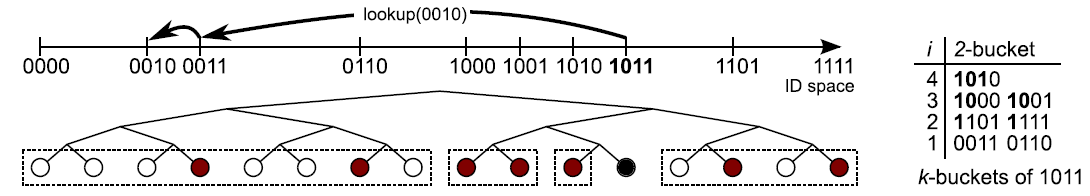
\includegraphics[width=0.9\linewidth]{images/kademlia_tree.png}
    \captionof{figure}{Visualisierung der Baumstruktur von Kademlia \parencite{MedranoChavez_ChordKademliaHighChurnScenarios}}
    \label{kademlia_tree}
\end{center}


\noindent Da bei einem Instant-Messaging-Protokoll häufig Teilnehmer das Netzwerk verlassen und neue Teilnehmer dem Netzwerk beitreten, ist es wichtig, dass das Protokoll mit hoher Fluktuation umgehen kann. Diese Fluktuation von Nodes wird als Churn (engl. Abwanderung) bezeichnet. In einer Studie von Medrano-Chávez et al. \parencite{MedranoChavez_ChordKademliaHighChurnScenarios}, welche im hybriden Journal \textit{Peer-to-Peer Networking and Applications} veröffentlicht wurde, wurde die Leistung von Chord und Kademlia in Bezug auf Netzwerkfluktuation untersucht. Die Ergebnisse zeigen, dass Kademlia bei hoher Fluktuation besser abschneidet als Chord. Aus diesem Grund wird Kademlia in diesem Protokoll als Grundlage für das Auffinden von Teilnehmern und das Routing verwendet.

% #TODO:Warum Kademlia und was die Sicherheitsaspekte angeht, erst in Architektur aufgreifen.
    % Signaling Server könnte auch mit Anfragen geflutet werden -> der Sever könnte bei jedem checken, ob es sich um einen validen Teilnehmer handelt, was aber sehr aufwändig wäre
    % wenn Kademlia mit Anfragen geflutet wird, könnte es zu einem Denial of Service kommen, da die Knoten nicht mehr erreichbar sind -> habe aber ja mit dem Signaling Server noch eine weitere Instanz, die die Anfragen entgegen nimmt und weiterleitet


% #TODO: Overlay Netzwerk erklären? Kademlia ist ein Overlay Netzwerk
\begin{itemize}
    \item Kademlia vs. Angriffe
    \item Angriffe gegen ICE gucken und erklären
\end{itemize}

\noindent Um die Problematik mit NATs zu lösen, wird das ICE-Protokoll verwendet. ICE ist ein Framework, das mehrere Techniken kombiniert, um eine Verbindung zwischen zwei Endpunkten herzustellen, die sich hinter NATs befinden. Genaue Details zur Implementierung von ICE folgt in Kapitel \ref{subsec:verbindungsmanagement} \textit{\nameref{subsec:verbindungsmanagement}}.


